\documentclass{standalone}

\begin{document}
	On se place dans le cadre du modèle \ref{model} et on suppose ainsi que l'on a $G \follows \Ger(N, p_A, p_B, p)$ avec $A$ et $B$ les communautés originelles et $\sigma$ l'étiquetage associé.
	
	On suppose sans perte de généralité que $p_A \leq p_B$. De plus on suppose que la probabilité qu'il y ait des arêtes inter-communauté est plus petit que la probabilité d'arêtes intra-classe: $2p \leq p_A + p_B$, autrement dit, on souhaite que le bruit dans le graphe ne soit pas trop important.
	
	\begin{thm}
		$\Proba[A:B \text{ est l'unique bissection minimale}] \underset{N \rightarrow \infty}{=} 1 + o(1)$
		\label{fonda}
	\end{thm}
	
	Pour démontrer ce résultat nous allons d'abord borner, pour $A':B'$, une bissection aléatoire, $\Proba [A':B' \prec A:B]$, pour borner par borne de l'union $\Proba [\exists A':B' / A':B' \prec A:B ]$ puis nous montrerons que cette borne tend vers $0$ rapidement.
	
	\begin{prop}
		Soit $A':B'$ une bissection de $G$ on a
		$\Proba [A':B' \prec A:B] \leq \exp\left(- \frac{2k(N-k)(p_a+p_b-2p)^2}{16 }\right)$.
		\label{borne1}
	\end{prop}
	\begin{proof}
				Soient $A'$, $B'$ une bissection de $G$, on a $\card{A'} = \card{B'} = N$.
		
		On veut comparer le flot des deux bissections $(A:B)$ et $A':B'$, on définit	\[ \Delta = \card{A':B'} - \card{A:B} \]
		On a $\Delta < 0$ si et seulement si $A':B'$ est une bissection plus petite que $(A:B)$; d'où $\Proba[A':B' \prec A:B] = \Proba[\Delta < 0]$.
		
		On va réécrire $\Delta$.
		
		Soient
		\begin{tabularx}{\textwidth}{llll}
			$A_1 = A \cap B'$  & $B_1 = B \cap B'$ & $A_2 = A \cap A'$ & $B_2 = B \cap A'$
		\end{tabularx}
		et $k=\card{A_1} = \card{B_2} $. Voir la figure~\ref{fig:patates}\footnote{Je pense que je mérite des points bonus rien que pour ces patates en Tikz.}. On peut supposer sans perte de généralité que $k \leq \frac12N$ quitte à permuter les notations. En effet, on a $B' = A_1 \sqcup B_1$ donc $\card{B'} = k + \card{B_1}$ et $\card{B_1} = N - k$ or
		$B = B_1 \sqcup B_2$ donc $\card{B} = \card{B_1} + \card{B_2}$ et $\card{B_2} = N - (N - k) = k$.
		
		De plus si $k \geq \frac12  N$, alors $\card{A_2} = N - k \leq \frac12 N$ et par le même raisonnement $B_1$ aussi. Il suffit de permuter les notation et d'échanger $A_1, A_2$ et $B_1, B_2$.
		
		\begin{figure}[H]
			
			\centering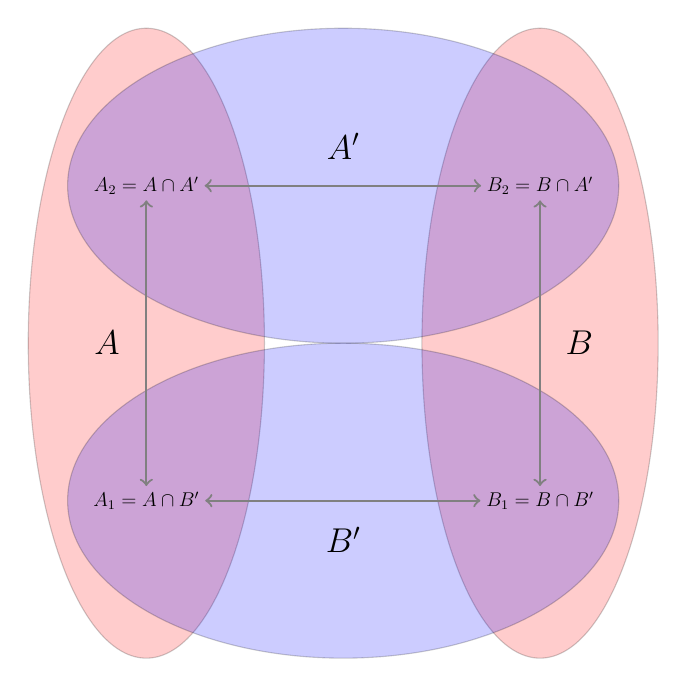
\begin{tikzpicture}[scale=0.5, every node/.style={scale=0.6}]
			
			\filldraw[fill=red, draw=black, opacity=0.2] (0,0) ellipse (3cm and 8cm); 
			\filldraw[fill=red, draw=black, opacity=0.2] (10,0) ellipse (3cm and 8cm);
			
			\filldraw[fill=blue, draw=black, opacity=0.2](5,4) ellipse (7cm and 4cm);
			
			\filldraw[fill=blue, draw=black, opacity=0.2](5,-4) ellipse (7cm and 4cm);
			
			\node (setA) at (-1,0) {\huge $A$};
			\node (setB) at (11,0) {\huge $B$};
			
			\node (setAp) at (5,5) {\huge $A'$};
			\node (setBp) at (5,-5) {\huge $B'$};
			
			\node (setA1) at (0,-4) {\large $A_1=A\cap B'$};
			\node (setA2) at (0,4) {\large $A_2=A\cap A'$};
			
			\node (setB1) at (10,-4) {\large $B_1=B\cap B'$};
			\node (setB2) at (10,4) {\large $B_2=B\cap A'$};
			
			\draw[color=gray, thick, <->] (setA1)  -- (setA2);
			\draw[color=gray, thick, <->] (setA2)  -- (setB2);
			\draw[color=gray, thick, <->] (setA1)  -- (setB1);
			\draw[color=gray, thick, <->] (setB1)  -- (setB2);
			
			\end{tikzpicture}
			
			\caption[Caption for LOF]{Représentation des 2 coupes considérées }
			\label{fig:patates}
		\end{figure}
		
		Et on remarque que:
		\begin{align*}
		A':B' &= (A \cap B'):(A \cap A') \sqcup (B \cap B':B \cap A') = (A_1:A_2) \sqcup (B_1:B_2) \\
		A:B &= (A \cap B'):(B \cap B') \sqcup (A \cap A':B \cap A') = (A_1:B_1) \sqcup (A_2:B_2) 
		\end{align*}
		Ainsi $\Delta = \card{A_1:A_2} + \card{B_1:B_2} - \card{A_1:B_1} - \card{A_2:B_2}$
		
		De plus dans le cadre de ce modèle on a $\card{A_1:B_1}, \card{A_2:B_2} \follows \Bin(k(m-k), p)$.
		
		En effet $\card{A_1:B_1}$ est le nombre d'arêtes présentes entre $A_1 = A \cap B'$ et $B_1 = B \cap B'$, il y a $\card{A_1} \times \card{B_1} = k(N-k)$ arêtes possibles entre ces deux ensembles. De plus, comme $A_1\subset A$ et $B_1\subset B$, chacune sont présentes avec probabilité $p$.
		
		Avec un raisonnement similaire on obtient que $\card{A1:A2} \follows \Bin(k(m-k), p_A)$ et $\card{B1:B2} \follows \Bin(k(m-k), p_B)$.
		
		On peut alors écrire $\Delta = \sum_{i=1}^{k(m-k)} \chi_i$ où les $\chi_i$ sont des variables aléatoires entières à valeurs dans $[-2, 2]$ et d'espérance $\Esp[\chi_i] = p_a+p_b-2p$.
		
		On va finalement pouvoir borner $\Proba [\Delta < 0]$ en utilisant l'inégalité de Hoeffding:
		\begin{align*}
		\Proba[\Delta < 0] = \Proba[\Delta - \Esp \Delta < - \Esp \Delta] &= \Proba[\Delta - \Esp \Delta < -k(N-k)(p_a+p_b-2p)] \\
		&\leq \exp\left(- \frac{2(k(N-k)(p_a+p_b-2p))^2}{\sum_{i=1}{k(n-k)} (2 +2)^2 }\right) \\
		&\leq \exp\left(- \frac{2k^2(N-k)^2(p_a+p_b-2p)^2}{k(n-k) 16 }\right) \\
		&\leq \exp\left(- \frac{2k(N-k)(p_a+p_b-2p)^2}{16 }\right)
		\end{align*}
	\end{proof}

	\begin{prop}
		$\Proba[A:B \text{ n'est pas la bissection minimale}] \leq \sum_{k=1}^{\lfloor \frac N2 \rfloor} \binom{N}{k}^2 \exp\left(- 2k(N-k)\lambda^2\right)$. \\$\text{Avec } \lambda =\frac{p_a+p_b-2p}{4 } > 0$.
		\label{borne2}
	\end{prop}

	\begin{proof} On va utiliser le proposition~\ref{borne1} pour contrôler: $\Proba[A:B \text{ n'est pas la bissection minimale}]$.
	\begin{align*}
	&\Proba[A:B \text{ n'est pas la bissection minimale}] = \Proba [\exists A':B' / A':B' \prec A:B ] \\ 
	& \leq \sum_{A':B' \text{une bissection}}\Proba[\Delta < 0] \\
			&= \sum_{k=1}^{\lfloor \frac N2 \rfloor} \binom{N}{k}^2 \Proba[\Delta < 0]  \\ 
			&\text{Pour définir une bissection il suffit de prendre $k$ éléments dans $A$} \\ 
			&\text{et $k$ éléments dans $B$ pour former $A'$, et cela fixe $B' = V \backslash A'$}.\\
			&\leq \sum_{k=1}^{\lfloor \frac N2 \rfloor} \binom{N}{k}^2 \exp\left(- \frac{2k(N-k)(p_a+p_b-2p)^2}{16 }\right)\\
		&\leq \sum_{k=1}^{\lfloor \frac N2 \rfloor} \binom{N}{k}^2 \exp\left(- 2k(N-k)\lambda^2\right) & \text{avec } \lambda =\frac{p_a+p_b-2p}{4 } > 0
	\end{align*}
	\end{proof}

	Nous allons maintenant montrer que cette borne tend vers $0$ lorsque $N$ grandit.

	\begin{prop}
		$\sum_{k=1}^{\lfloor \frac N2 \rfloor} \binom{N}{k}^2 \exp\left(- 2k(N-k)\lambda^2\right) \underset{N \rightarrow \infty}{=} \Orond\left(N^2 \exp\left(- 2N\lambda^2\right)\right)$ 
		\\ $\text{avec } \lambda =\frac{p_a+p_b-2p}{4 } > 0$
	\end{prop}

	\begin{proof}
	
	On remarque tout d'abord que $\lambda \in ]0, \frac12]$ et $\lambda^2 \in ]0, \frac14]$, posons alors $p = \left\lceil \frac{4}{\lambda^2}\right\rceil \geq 16$.
	
	On va alors scinder la somme en deux en conservant d'un côté les $p-1$ premiers termes et les autres de l'autre.
	
	On a:
	\begin{align*}
		\sum_{k=1}^{p-1} \binom{N}{k}^2 \exp\left(- 2k(N-k)\lambda^2\right) &\leq \sum_{k=1}^{p-1} N^{2k} \exp\left(- 2k(N-p+1)\lambda^2\right) \\
			&\leq N^{2} \exp\left(- 2(N-p+1)\lambda^2\right) \sum_{k=0}^{p-2} \left(N^{2} \exp\left(- 2k(N-p+1)\lambda^2\right)\right)^k \\
			&= \Orond\left(N^2 \exp\left(- 2N\lambda^2\right)\right)
	\end{align*}
	Maintenant on va montrer que le reste de la somme est négligeable.
	
	\begin{align*}
		\sum_{k=p}^{\lfloor \frac N2 \rfloor} \binom{N}{k}^2 \exp\left(- 2k(N-k)\lambda^2\right) &\leq \frac N2 4^N \exp\left( - p  \frac N2 \lambda^2 \right) & \text{car } \binom{N}{k} \leq 2^N \\
		&= \frac N2 \left( 4 \exp\left( - p  \frac N2 \lambda^2 \right) \right)^N
	\end{align*}
	
	Or puisque $p \geq 16$ et $\lambda \in ]0, 1/2]$, on a $4 \exp\left( - p  \frac 2 \lambda^2 \right) \leq 4 \exp\left( - \frac {16}{2} \lambda^2 \right) = 4 \exp\left( - 8 \lambda^2 \right) \leq \exp(- \lambda^2)$
	
	On conclut donc que $ \sum_{k=p}^{\lfloor \frac N2 \rfloor} \binom{N}{k}^2 \exp\left(- 2k(N-k)\lambda^2\right) \underset{N \rightarrow \infty}{=} o\left(N^2 \exp\left(- 2N\lambda^2\right)\right)$.
	
	Ainsi on obtient finalement $\Proba[A:B \text{ n'est pas la bissection minimale}] \underset{N \rightarrow \infty}{=} \Orond\left(N^2 \exp\left(- 2N\lambda^2\right)\right)$
	\end{proof}

	On peut alors prouver le théorème~\ref{fonda} par application successive de ces 3 résultats.
	
	On a obtenu 
	\begin{align*}
		\Proba[A:B \text{ n'est pas la bissection minimale}] &\leq \sum_{k=1}^{\lfloor \frac N2 \rfloor} \binom{N}{k}^2 \exp\left(- 2k(N-k)\lambda^2\right) \\
		&\underset{N \rightarrow \infty}{=} \Orond\left(N^2 \exp\left(- 2N\lambda^2\right)\right)
	\end{align*}
	
	Et on peut donc conclure:
	\begin{align*}
	\Proba[A:B \text{ est la bissection minimale}] &= 1-\Proba[A:B \text{ n'est pas la bissection minimale}] \\ 
	&\underset{N \rightarrow \infty}{=} 1-o(1)
	\end{align*}

	Ainsi on peut ramener le problème de reconstruction exacte de communauté à la recherche d'une bissection minimale qui sera alors avec grande probabilité la paire de communautés recherchée. 

\end{document}
